\section*{Problem 1}
	\begin{proof} [Solution]
		Let take the observation day $T = 1000$ and plot the result.\\
		\begin{center}
			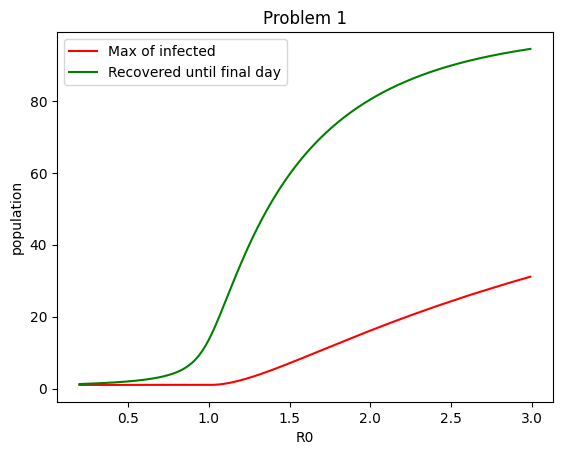
\includegraphics[scale=0.7]{Problem1.png}
		\end{center}
		Here, we can observe that each graph is changed dramatically around $R_0 = 1$. Note that $R_0 = \frac{\beta}{\gamma}.$ If $R_0 > 1$, then it follows $\beta > \gamma$. This means the initial infected person meet some people before recovering. Then infection may occur in other people and they again spread, so it leads to pandemic. If $R_0 < 1$, then it follows $\beta < \gamma$. This means the initial infected person meet some people after(or end of) recovering. Then infection may not occur in other people so the spread of disease does not last long. By using this observation, we can get some strategies to mitigate the pandemic: Isolate the infected person until he or she recover completely and reduce opportunities for contact.\\
	\end{proof}